% ============================================================================
%  Reliable 3D — World-Class Academic Poster
%  Title: Enhancing Robustness of Point Cloud Models to Attacks and Corruptions
% ============================================================================
\documentclass[25pt, a0paper, landscape]{tikzposter}

% ── Packages ────────────────────────────────────────────────────────────────
\usepackage[T1]{fontenc}
\usepackage{lmodern}
\usepackage{amsmath,amssymb}
\usepackage{booktabs}
\usepackage{enumitem}
\usepackage{graphicx}
\usepackage{multicol}
\usepackage{xcolor}
\usepackage{tikz}
\usetikzlibrary{arrows.meta, positioning, shapes.geometric, calc, fit, decorations.pathreplacing}
\usepackage{tcolorbox}
\tcbuselibrary{skins}

% ── Color Palette (deep navy + accent teal + warm highlights) ───────────────
\definecolor{PrimaryDark}{HTML}{0D1B2A}
\definecolor{PrimaryMid}{HTML}{1B2A4A}
\definecolor{AccentTeal}{HTML}{0097A7}
\definecolor{AccentCyan}{HTML}{00BCD4}
\definecolor{Highlight}{HTML}{FF6F00}
\definecolor{HighlightGreen}{HTML}{43A047}
\definecolor{LightBg}{HTML}{F5F7FA}
\definecolor{CardBg}{HTML}{FFFFFF}
\definecolor{TextDark}{HTML}{1A1A2E}
\definecolor{TextMuted}{HTML}{546E7A}
\definecolor{ResultRed}{HTML}{E53935}
\definecolor{ResultGreen}{HTML}{2E7D32}
\definecolor{ResultBlue}{HTML}{1565C0}
\definecolor{PipelineArrow}{HTML}{0097A7}
\definecolor{BoxBorder}{HTML}{B0BEC5}
\definecolor{SoftGold}{HTML}{F9A825}

% ── Poster Theme ────────────────────────────────────────────────────────────
\usetheme{Default}
\definecolorstyle{ReliableStyle}{
  \colorlet{colorOne}{PrimaryDark}
  \colorlet{colorTwo}{AccentTeal}
  \colorlet{colorThree}{LightBg}
}{
  % Background
  \colorlet{backgroundcolor}{LightBg}
  \colorlet{framecolor}{PrimaryDark}
  % Title
  \colorlet{titlefgcolor}{white}
  \colorlet{titlebgcolor}{PrimaryDark}
  % Block
  \colorlet{blocktitlebgcolor}{PrimaryMid}
  \colorlet{blocktitlefgcolor}{white}
  \colorlet{blockbodybgcolor}{CardBg}
  \colorlet{blockbodyfgcolor}{TextDark}
  % Inner block
  \colorlet{innerblocktitlebgcolor}{AccentTeal}
  \colorlet{innerblocktitlefgcolor}{white}
  \colorlet{innerblockbodybgcolor}{LightBg}
  \colorlet{innerblockbodyfgcolor}{TextDark}
}
\usecolorstyle{ReliableStyle}

\useblockstyle{Default}
\useinnerblockstyle{Default}

% Rounded blocks
\defineblockstyle{RoundedBlock}{
  titlewidthscale=1.0,
  bodywidthscale=1.0,
  titleleft,
  titleoffsetx=0pt,
  titleoffsety=0pt,
  bodyoffsetx=0pt,
  bodyoffsety=0pt,
  bodyverticalshift=0pt,
  roundedcorners=16,
  linewidth=2pt,
  titleinnersep=10mm,
  bodyinnersep=10mm
}{
  \draw[rounded corners=\blockroundedcorners, inner sep=\blockbodyinnersep,
        line width=\blocklinewidth, color=blocktitlebgcolor,
        fill=blockbodybgcolor]
    (blockbody.south west) rectangle (blockbody.north east);
  \ifBlockHasTitle
    \draw[rounded corners=\blockroundedcorners, inner sep=\blocktitleinnersep,
          line width=\blocklinewidth, color=blocktitlebgcolor,
          fill=blocktitlebgcolor]
      (blocktitle.south west) rectangle (blocktitle.north east);
  \fi
}
\useblockstyle{RoundedBlock}

% ── Title Formatting ───────────────────────────────────────────────────────
\settitle{
  \centering
  \vbox{
    \centering
    \color{titlefgcolor}
    {\bfseries\Huge\sc Reliable 3D: Enhancing Robustness of Point Cloud\\[0.3em] Models to Attacks and Corruptions\par}
    \vspace{14mm}
    {\LARGE Saif Al-Din Ali\textsuperscript{1} \quad Rosina Kharal\textsuperscript{2} \quad Abu Bakr Nafees\textsuperscript{3}\par}
    \vspace{6mm}
    {\large \textsuperscript{1,2}University of Waterloo, Ontario, Canada \qquad \textsuperscript{3}Independent Researcher\par}
    \vspace{4mm}
    {\normalsize \texttt{\{sa29ali, rkharal\}@uwaterloo.ca \quad abubakr@nafees.ca}\par}
  }
}

% ── Macros ──────────────────────────────────────────────────────────────────
\newcommand{\statbox}[3]{%
  \begin{tcolorbox}[
    colback=#1!8, colframe=#1, boxrule=2pt,
    arc=10pt, boxsep=5pt,
    width=0.95\linewidth, halign=center,
    top=4mm, bottom=4mm
  ]
    {\fontsize{52}{58}\selectfont\bfseries\color{#1}#2}\\[3mm]
    {\large\color{TextDark}#3}
  \end{tcolorbox}%
}

\newcommand{\resultrow}[4]{%
  #1 & #2 & \textcolor{ResultRed}{#3} & \textcolor{ResultGreen}{\textbf{#4}} \\
}

\newcommand{\ccmark}{\textcolor{HighlightGreen}{\textbf{\checkmark}}}
\newcommand{\xxmark}{\textcolor{ResultRed}{\textbf{\texttimes}}}

% ============================================================================
\begin{document}
\maketitle[width=0.98\textwidth, titletotopverticalspace=10mm, titletoblockverticalspace=14mm]

% ############################################################################
%  ROW 1 — Left Column
% ############################################################################
\begin{columns}

% ════════════════════════════════════════════════════════════════════════════
%  COLUMN 1 (left)
% ════════════════════════════════════════════════════════════════════════════
\column{0.25}

% ── Motivation & Problem ───────────────────────────────────────────────────
\block{1. Motivation \& Problem}{
  \large
  3D point cloud perception is \textbf{mission-critical} for autonomous vehicles, robotics, and AR/VR systems. Yet, real-world deployments face:

  \vspace{6mm}
  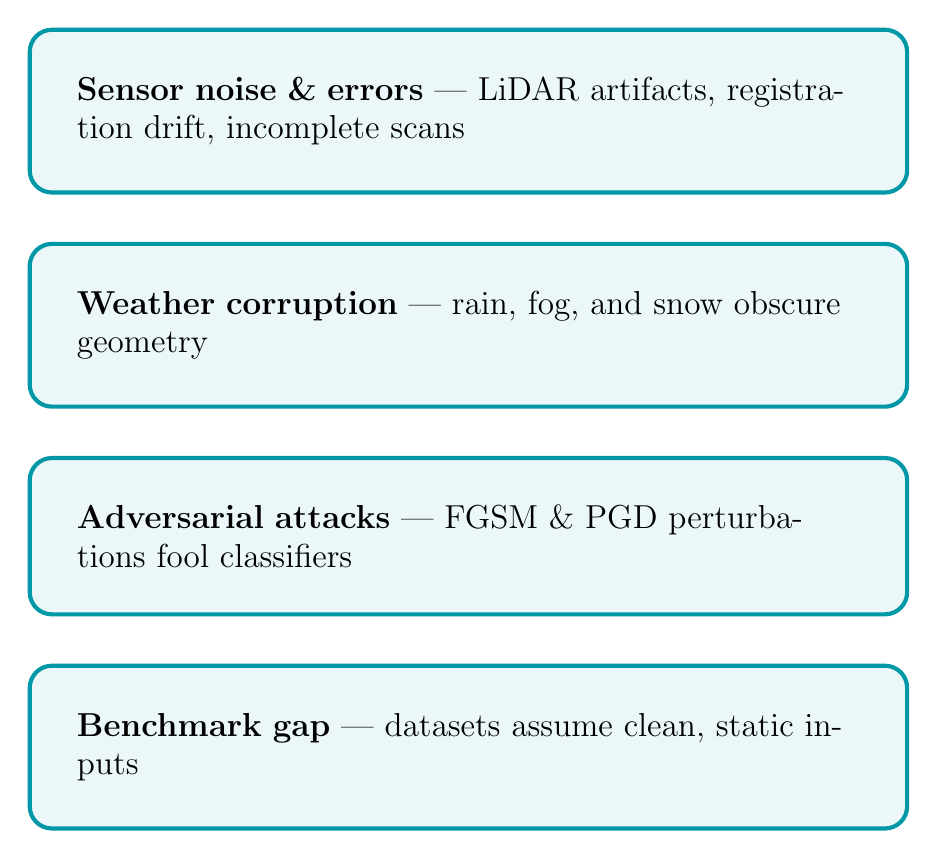
\begin{tikzpicture}[
    every node/.style={font=\large},
    prob/.style={
      draw=AccentTeal, fill=AccentTeal!8, rounded corners=8pt,
      minimum width=0.88\linewidth, minimum height=18mm,
      text width=0.82\linewidth, align=left, inner sep=6mm,
      line width=1.5pt
    }
  ]
    \node[prob] (a) at (0,0)  {\textbf{Sensor noise \& errors} — LiDAR artifacts, registration drift, incomplete scans};
    \node[prob, below=6mm of a] (b) {\textbf{Weather corruption} — rain, fog, and snow obscure geometry};
    \node[prob, below=6mm of b] (c) {\textbf{Adversarial attacks} — FGSM \& PGD perturbations fool classifiers};
    \node[prob, below=6mm of c] (d) {\textbf{Benchmark gap} — datasets assume clean, static inputs};
  \end{tikzpicture}

  \vspace{6mm}
  \begin{center}
    \begin{tcolorbox}[
      colback=Highlight!8, colframe=Highlight, boxrule=2.5pt,
      arc=12pt, width=0.92\linewidth, halign=center,
      top=4mm, bottom=4mm
    ]
      {\Large\bfseries\color{Highlight} Distortions cause up to a 30\% accuracy drop\\[2mm] in state-of-the-art 3D classifiers.}
    \end{tcolorbox}
  \end{center}

  \vspace{3mm}
  {\large\color{TextMuted} Robustness in 3D point clouds remains \textbf{highly underexplored} compared to 2D vision, despite widespread safety-critical deployment.}
}

% ── Corruption Types ──────────────────────────────────────────────────────
\block{2. Corruption \& Attack Taxonomy}{
  \large

  \vspace{2mm}
  \innerblock{\large\bfseries Sensory \& Weather Corruptions}{
    \begin{itemize}[leftmargin=8mm, itemsep=3mm, labelsep=4mm]
      \item[\textcolor{AccentTeal}{\large$\blacktriangleright$}] \textbf{Occlusion} — random removal of geometry (obstruction, incomplete scans)
      \item[\textcolor{AccentTeal}{\large$\blacktriangleright$}] \textbf{LiDAR noise} — spurious points from sensor imperfections
      \item[\textcolor{AccentTeal}{\large$\blacktriangleright$}] \textbf{Registration error} — random rotation/translation from misaligned scans
      \item[\textcolor{AccentTeal}{\large$\blacktriangleright$}] \textbf{Rain} — regularly spaced artifacts along all axes
    \end{itemize}
  }

  \vspace{6mm}
  \innerblock{\large\bfseries Adversarial Attacks}{
    \begin{itemize}[leftmargin=8mm, itemsep=3mm, labelsep=4mm]
      \item[\textcolor{Highlight}{\large$\blacktriangleright$}] \textbf{FGSM} — Fast Gradient Sign Method (single-step white-box)
      \item[\textcolor{Highlight}{\large$\blacktriangleright$}] \textbf{PGD} — Projected Gradient Descent (iterative white-box)
      \item[\textcolor{Highlight}{\large$\blacktriangleright$}] \textbf{Combined} — adversarial + weather corruption simultaneously
    \end{itemize}
  }

  \vspace{4mm}
  \begin{center}
    \small\color{TextMuted}
    \textit{All corruptions are simulated on clean ModelNet40 point clouds to replicate physically realistic conditions.}
  \end{center}
}

% ════════════════════════════════════════════════════════════════════════════
%  COLUMN 2 (center-left)
% ════════════════════════════════════════════════════════════════════════════
\column{0.25}

% ── Proposed Method ───────────────────────────────────────────────────────
\block{3. Combined Corrective Function Pipeline (CCF)}{
  \large
  We propose a \textbf{three-stage defense pipeline} where each corrective function operates at a distinct phase, ensuring \textbf{zero mutual interference}:

  \vspace{8mm}
  \begin{center}
  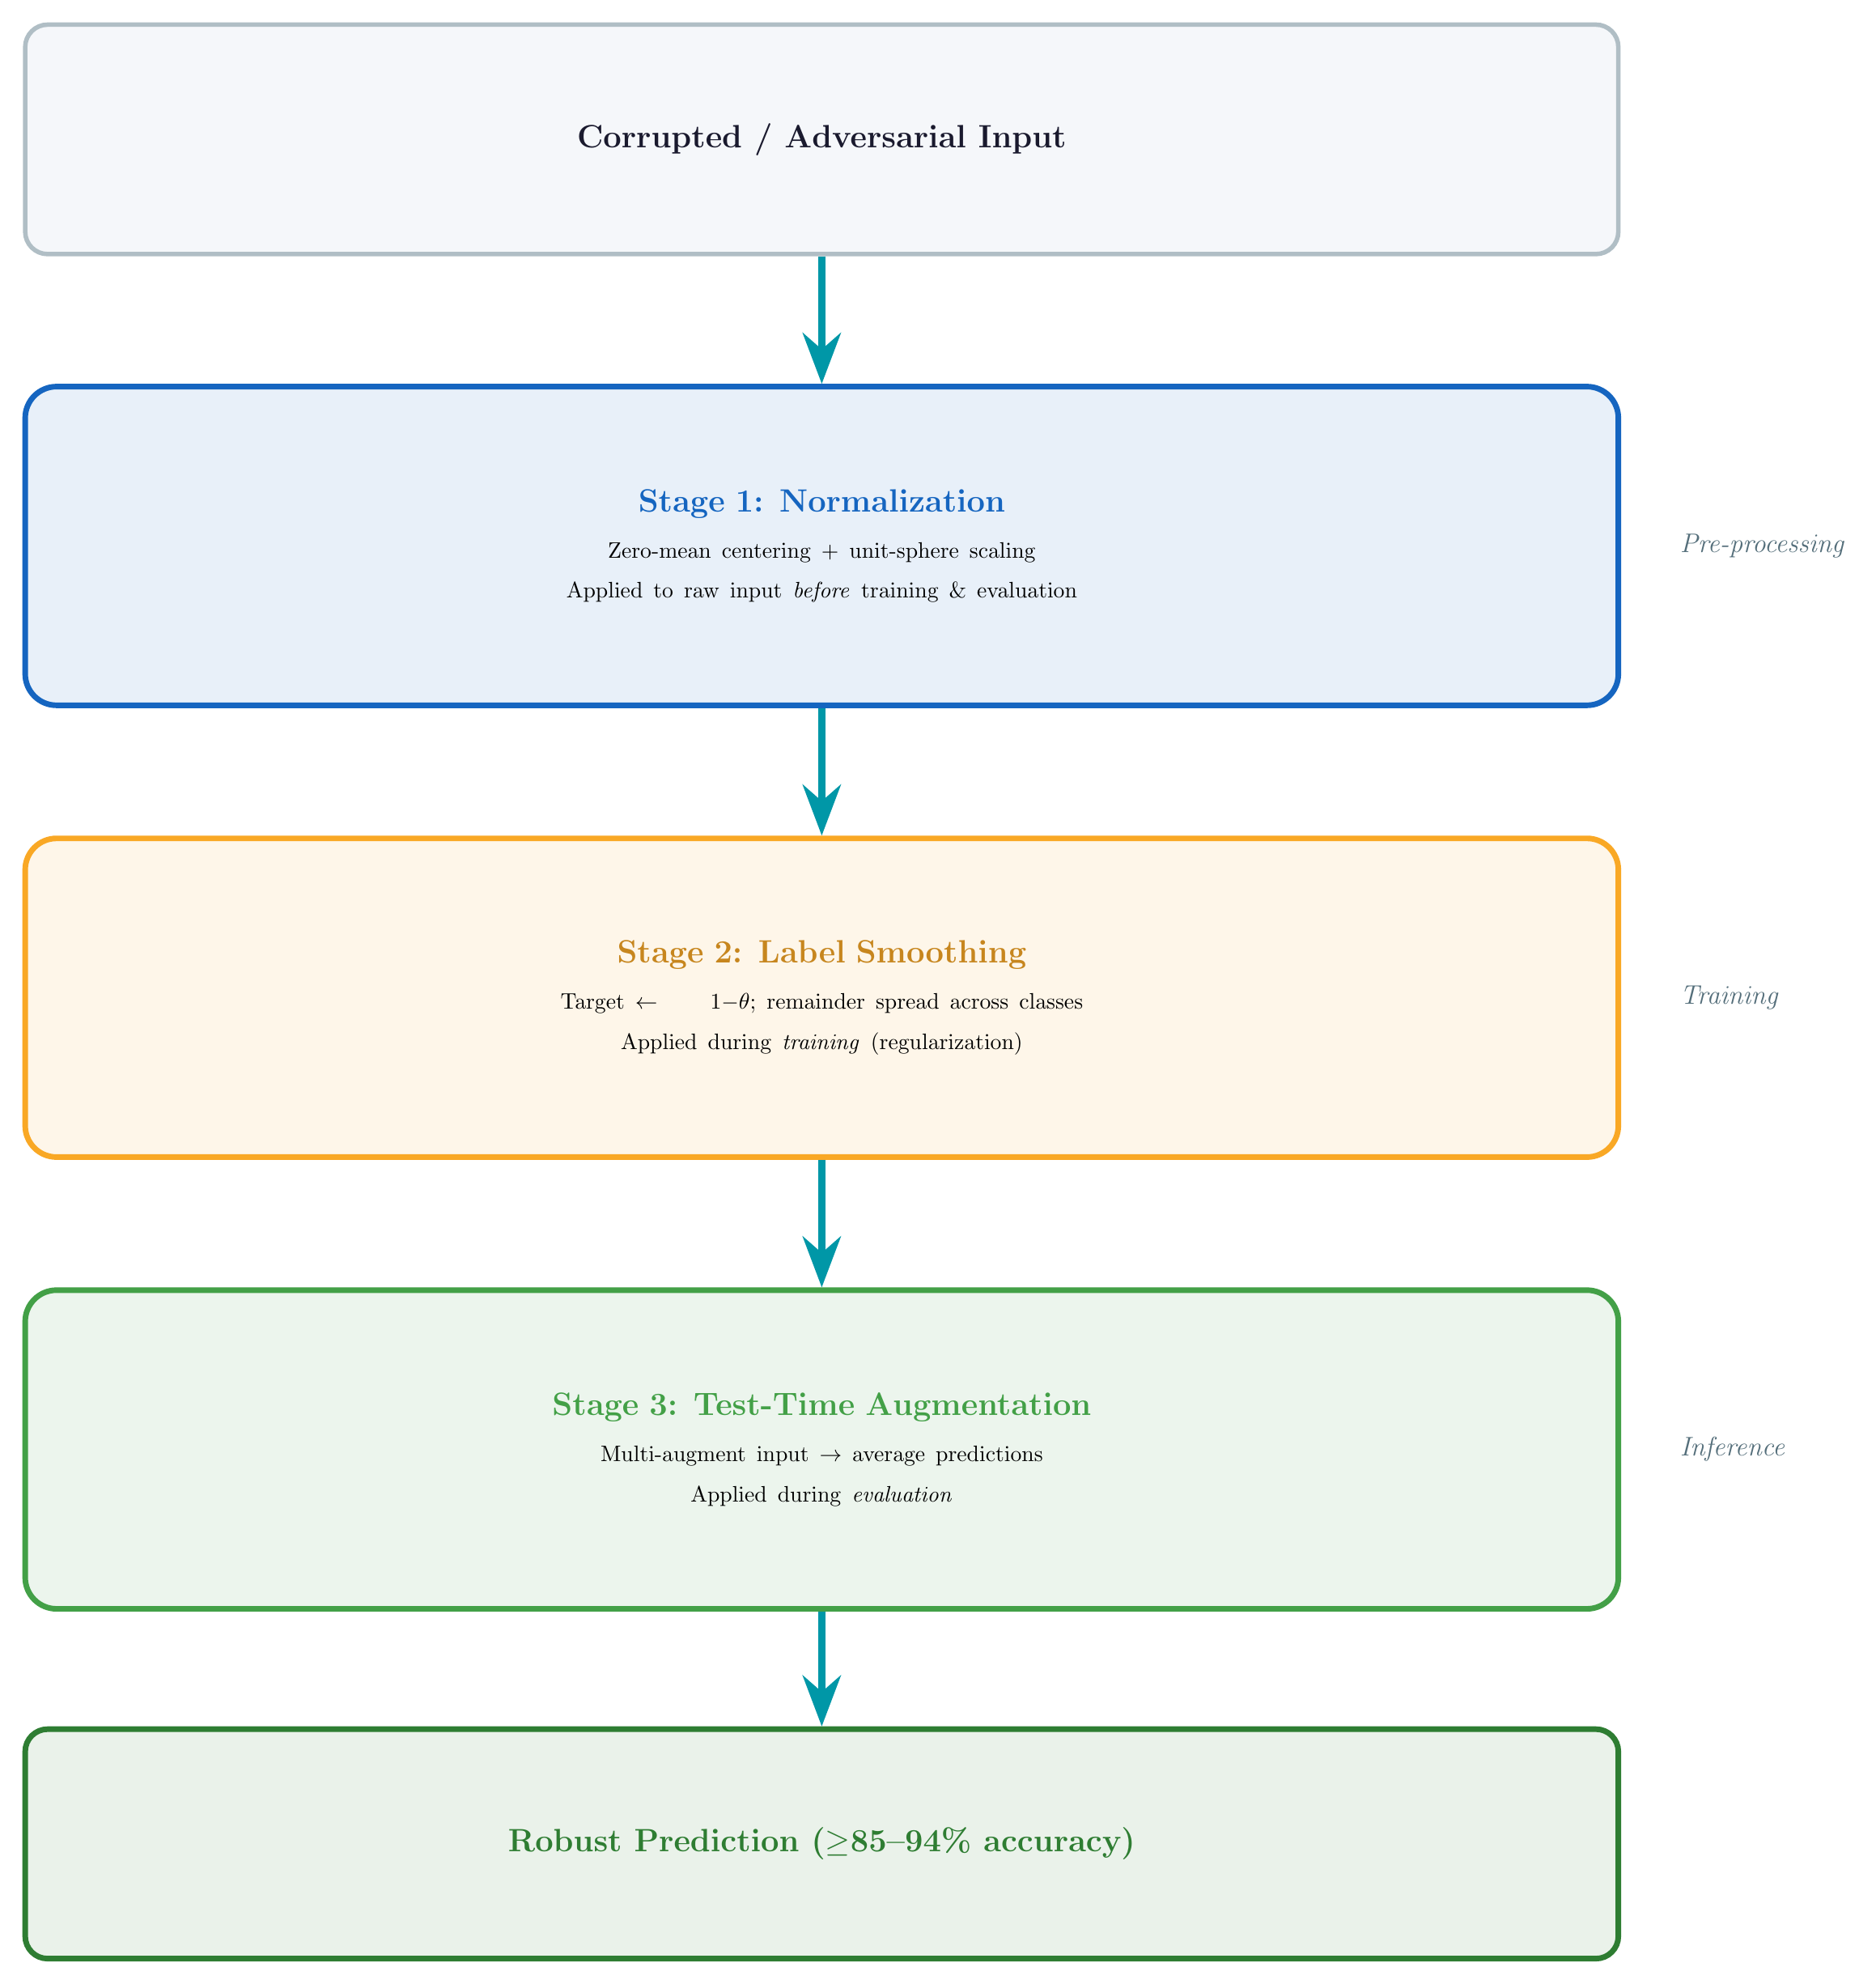
\begin{tikzpicture}[
    stage/.style={
      draw=#1, fill=#1!10, rounded corners=14pt,
      minimum width=250mm, minimum height=50mm,
      text width=230mm, align=center, inner sep=6mm,
      line width=2.5pt, font=\Large
    },
    arr/.style={-{Stealth[length=8mm,width=6mm]}, line width=3pt, color=PipelineArrow},
    lbl/.style={font=\large\color{TextMuted}, anchor=west}
  ]
    % Input
    \node[draw=BoxBorder, fill=LightBg, rounded corners=10pt,
          minimum width=250mm, minimum height=36mm, align=center,
          line width=2pt, font=\Large\bfseries] (input) at (0, 0)
      {\color{TextDark}Corrupted / Adversarial Input};

    % Stage 1
    \node[stage=ResultBlue, below=20mm of input] (s1)
      {\textbf{\color{ResultBlue}Stage 1: Normalization}\\[3mm]
       \normalsize Zero-mean centering + unit-sphere scaling\\
       Applied to raw input \textit{before} training \& evaluation};

    % Stage 2
    \node[stage=SoftGold, below=20mm of s1] (s2)
      {\textbf{\color{SoftGold!80!black}Stage 2: Label Smoothing}\\[3mm]
       \normalsize Target $\leftarrow 1{-}\theta$; remainder spread across classes\\
       Applied during \textit{training} (regularization)};

    % Stage 3
    \node[stage=HighlightGreen, below=20mm of s2] (s3)
      {\textbf{\color{HighlightGreen}Stage 3: Test-Time Augmentation}\\[3mm]
       \normalsize Multi-augment input $\rightarrow$ average predictions\\
       Applied during \textit{evaluation}};

    % Output
    \node[draw=ResultGreen, fill=ResultGreen!10, rounded corners=10pt,
          minimum width=250mm, minimum height=36mm, align=center,
          line width=2.5pt, font=\Large\bfseries, below=18mm of s3] (output)
      {\color{ResultGreen}Robust Prediction ($\geq$85--94\% accuracy)};

    % Arrows
    \draw[arr] (input)  -- (s1);
    \draw[arr] (s1)     -- (s2);
    \draw[arr] (s2)     -- (s3);
    \draw[arr] (s3)     -- (output);

    % Phase labels
    \node[lbl] at ($(s1.east)+(8mm,0)$) {\textit{Pre-processing}};
    \node[lbl] at ($(s2.east)+(8mm,0)$) {\textit{Training}};
    \node[lbl] at ($(s3.east)+(8mm,0)$) {\textit{Inference}};
  \end{tikzpicture}
  \end{center}

  \vspace{5mm}
  \begin{center}
    \begin{tcolorbox}[
      colback=AccentTeal!6, colframe=AccentTeal, boxrule=2pt,
      arc=10pt, width=0.92\linewidth, halign=center,
      top=3mm, bottom=3mm
    ]
      {\large\bfseries\color{PrimaryDark}
        Simple $\bullet$ Fast $\bullet$ No retraining from scratch $\bullet$ Composable}
    \end{tcolorbox}
  \end{center}
}

% ════════════════════════════════════════════════════════════════════════════
%  COLUMN 3 (center-right)
% ════════════════════════════════════════════════════════════════════════════
\column{0.25}

% ── Dataset & Experimental Setup ──────────────────────────────────────────
\block{4. Dataset \& Experimental Setup}{
  \large

  \innerblock{\normalsize\bfseries Dataset}{
    \begin{itemize}[leftmargin=8mm, itemsep=2mm, labelsep=4mm]
      \item[\textcolor{AccentTeal}{\large$\bullet$}]
        \textbf{ModelNet40} — 12,311 CAD models across 40 categories, converted to \textbf{point cloud} form
      \item[\textcolor{AccentTeal}{\large$\bullet$}]
        Point clouds chosen over meshes for \textbf{memory efficiency} and ease of corruption simulation
      \item[\textcolor{AccentTeal}{\large$\bullet$}]
        \textbf{Baseline accuracy} (clean, no CCF): \textbf{71.9\%}
    \end{itemize}
  }

  \vspace{4mm}
  \innerblock{\normalsize\bfseries Protocol}{
    \begin{itemize}[leftmargin=8mm, itemsep=2mm, labelsep=4mm]
      \item[\textcolor{AccentTeal}{\large$\bullet$}]
        \textbf{4 corruption types} simulated at realistic severity
      \item[\textcolor{AccentTeal}{\large$\bullet$}]
        \textbf{2 white-box attacks:} FGSM (single-step) \& PGD (iterative)
      \item[\textcolor{AccentTeal}{\large$\bullet$}]
        \textbf{Combined attack:} FGSM + rain simultaneously
      \item[\textcolor{AccentTeal}{\large$\bullet$}]
        Each CF tested individually \& as full \textbf{CCF pipeline}; also on \textbf{clean data}
    \end{itemize}
  }
}

% ── Key Results ───────────────────────────────────────────────────────────
\block{5. Key Results}{
  \large

  \vspace{2mm}
  \innerblock{\large\bfseries A. Corruption Robustness}{
    \vspace{4mm}
    \begin{center}
    \renewcommand{\arraystretch}{1.5}
    \begin{tabular}{@{} l c c c @{}}
      \toprule
      \textbf{Corruption} & \textbf{No CF} & \textbf{Best Single CF} & \textbf{CCF} \\
      \midrule
      Occlusion          & \textcolor{ResultRed}{42\%}  & 74\%  & \textcolor{ResultGreen}{\textbf{84\%}} \\
      LiDAR Noise        & \textcolor{ResultRed}{47\%}  & 78\%  & \textcolor{ResultGreen}{\textbf{84\%}} \\
      Registration Error & \textcolor{ResultRed}{52\%}  & 92\%  & \textcolor{ResultGreen}{\textbf{94\%}} \\
      Rain               & \textcolor{ResultRed}{52\%}  & 72\%  & \textcolor{ResultGreen}{\textbf{79\%}} \\
      \midrule
      Clean (no attack)  & 72\%  & 83\%  & \textcolor{ResultGreen}{\textbf{94\%}} \\
      \bottomrule
    \end{tabular}
    \end{center}
    \vspace{2mm}
    \begin{center}
      \small\color{TextMuted}\textit{CCF restores accuracy to $\geq$79\% in all corrupted cases and boosts clean accuracy by +22\%.}
    \end{center}
  }

  \vspace{8mm}
  \innerblock{\large\bfseries B. Adversarial Robustness}{
    \vspace{4mm}
    \begin{center}
    \renewcommand{\arraystretch}{1.5}
    \begin{tabular}{@{} l c c @{}}
      \toprule
      \textbf{Attack} & \textbf{No Defense} & \textbf{With CCF} \\
      \midrule
      FGSM            & \textcolor{ResultRed}{39.5\%} & \textcolor{ResultGreen}{\textbf{94\%}} \\
      PGD             & \textcolor{ResultRed}{40\%}   & \textcolor{ResultGreen}{\textbf{94\%}} \\
      FGSM + Rain     & \textcolor{ResultRed}{56.6\%} & \textcolor{ResultGreen}{\textbf{93\%}} \\
      \bottomrule
    \end{tabular}
    \end{center}
    \vspace{2mm}
    \begin{center}
      \small\color{TextMuted}\textit{CCF yields up to \textbf{+54\%} accuracy gain under adversarial attack.}
    \end{center}
  }

}

% ════════════════════════════════════════════════════════════════════════════
%  COLUMN 4 (right)
% ════════════════════════════════════════════════════════════════════════════
\column{0.25}

% ── Headline Stats ───────────────────────────────────────────────────────
\block{}{%
  \begin{center}
  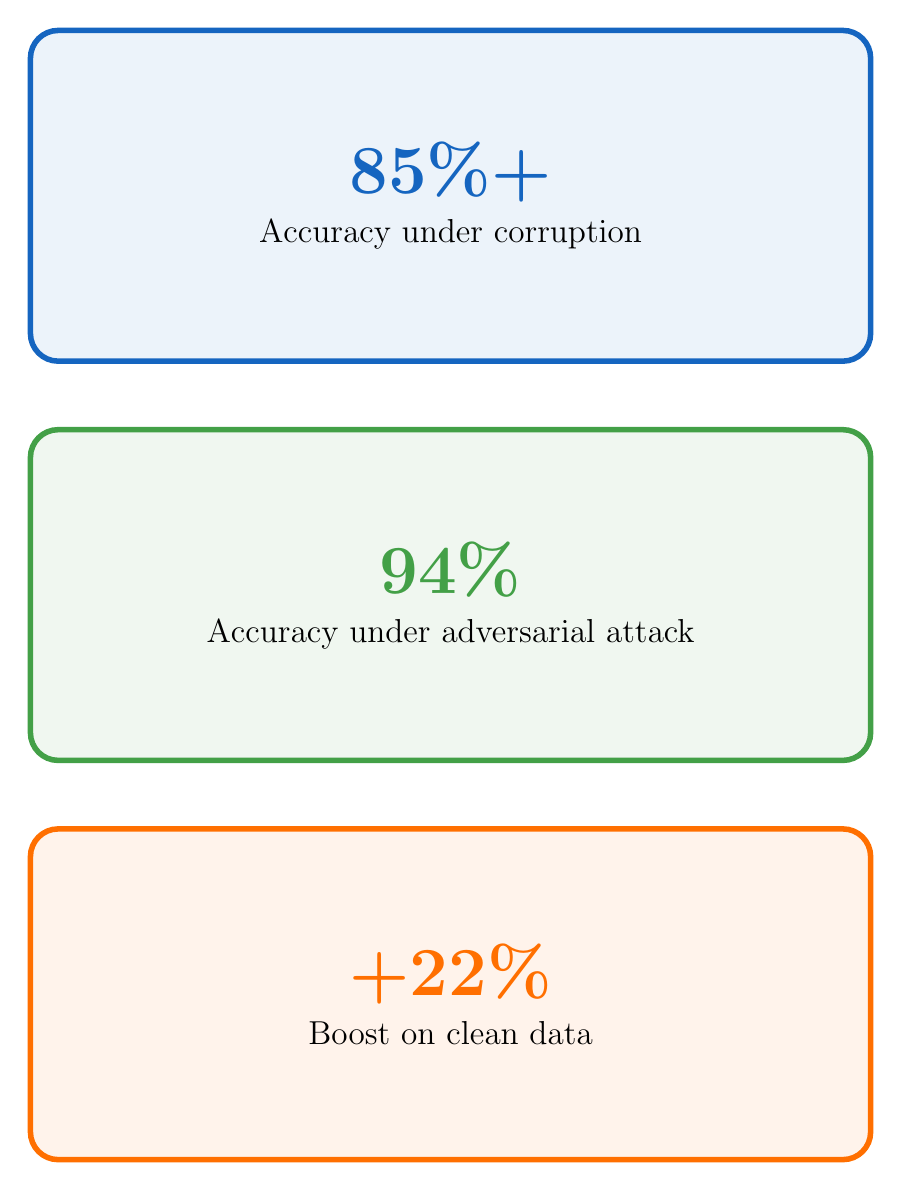
\begin{tikzpicture}[
    stat/.style={
      rounded corners=10pt, minimum width=0.88\linewidth, minimum height=42mm,
      align=center, inner sep=4mm, line width=2pt
    }
  ]
    \node[stat, draw=ResultBlue, fill=ResultBlue!8] (s1) at (0,0) {
      {\fontsize{42}{48}\selectfont\bfseries\color{ResultBlue}85\%+}\\[2mm]
      {\large Accuracy under corruption}
    };
    \node[stat, draw=HighlightGreen, fill=HighlightGreen!8, below=8mm of s1] (s2) {
      {\fontsize{42}{48}\selectfont\bfseries\color{HighlightGreen}94\%}\\[2mm]
      {\large Accuracy under adversarial attack}
    };
    \node[stat, draw=Highlight, fill=Highlight!8, below=8mm of s2] (s3) {
      {\fontsize{42}{48}\selectfont\bfseries\color{Highlight}+22\%}\\[2mm]
      {\large Boost on clean data}
    };
  \end{tikzpicture}
  \end{center}
}

% ── Why It Works ─────────────────────────────────────────────────────────
\block{6. Why CCF Works}{
  \large
  \begin{enumerate}[leftmargin=8mm, itemsep=4mm, labelsep=4mm]
    \item \textbf{Normalization} removes positional/scale bias introduced by sensor drift and corruption
    \item \textbf{Label smoothing} prevents overconfidence on noisy training signals, improving generalization
    \item \textbf{TTA} averages out stochastic distortion effects at inference
    \item The three stages are \textbf{orthogonal} — each targets a different pipeline phase with no interference
  \end{enumerate}

  \vspace{4mm}
  \begin{center}
    \small\color{TextMuted}\textit{Minimal computational overhead — suitable for real-time deployment.}
  \end{center}
}

% ── Conclusions & Future Work ─────────────────────────────────────────────
\block{7. Conclusions \& Future Directions}{
  \large
  \innerblock{\normalsize\bfseries Key Takeaways}{
    \begin{itemize}[leftmargin=8mm, itemsep=3mm, labelsep=4mm]
      \item[\ccmark] CCF restores and \textit{exceeds} baseline accuracy under all tested distortions
      \item[\ccmark] No degradation on clean data — in fact, \textbf{+22\%} improvement
      \item[\ccmark] Surpasses state-of-the-art both for corruption and adversarial defense
      \item[\ccmark] Lightweight, composable, and easy to integrate into existing systems
    \end{itemize}
  }

  \vspace{6mm}
  \innerblock{\normalsize\bfseries Future Work}{
    \begin{itemize}[leftmargin=8mm, itemsep=3mm, labelsep=4mm]
      \item[\textcolor{AccentCyan}{$\triangleright$}] Adaptive pipeline — dynamically weight CFs based on corruption severity
      \item[\textcolor{AccentCyan}{$\triangleright$}] Expand to black-box attacks, data poisoning, and physical-world spoofing
      \item[\textcolor{AccentCyan}{$\triangleright$}] Validate on ShapeNet, KITTI, and nuScenes for diverse real-world coverage
      \item[\textcolor{AccentCyan}{$\triangleright$}] End-to-end deployment in autonomous perception--planning--control stack
    \end{itemize}
  }
}

% ── References ────────────────────────────────────────────────────────────
\block{References}{
  \small
  \begin{enumerate}[leftmargin=6mm, itemsep=1mm, labelsep=3mm]
    \item Li et al., ``Common Corruption Robustness of Point Cloud Detectors,'' \textit{ECCV Workshop}, 2024.
    \item Huang et al., ``Improving Robustness of LiDAR-Camera Fusion Against Weather Corruption,'' \textit{IEEE T-IV}, 2024.
    \item Sun et al., ``Adversarial Robustness of 3D Point Cloud Classification: A Geometric Perspective,'' \textit{ICML}, 2023.
    \item Goodfellow et al., ``Explaining and Harnessing Adversarial Examples'' (FGSM), \textit{ICLR}, 2015.
    \item Madry et al., ``Towards Deep Learning Models Resistant to Adversarial Attacks'' (PGD), \textit{ICLR}, 2018.
    \item Wu et al., ``3D ShapeNets / ModelNet40,'' \textit{CVPR}, 2015.
  \end{enumerate}
}

\end{columns}

\end{document}
